%% ==============================
\chapter{\iflanguage{ngerman}{Design}{Concept}}
\label{sec:concept}
%% ==============================


\todo{Formulierung}

Das hier folgende Kapitel beschäftigt sich mit dem Softwaredesign der Implementierung dieser Arbeit.
\newline
Die hier vorgestellte Implementierung teilt sich dabei in zwei verschieden Programme auf. Zum einen den sogenannten \textit{VolumeRenderHelper}, der für das Laden, Umwandeln, Verarbeiten und Speichern der Volumendaten zuständig ist. Auf der anderen Seite das Unityprogramm \textit{VolumeRenderer}, welches zur Visualisierung der vom Helper erzeugten Daten dient. Diese beiden Programme existierten bereits vorher und sind in Vorarbeiten des IPRs entstanden. In dieser Arbeit wurde der \textit{VolumeRenderHelper} um die vorgestellte Transferfunktion und der \textit{VolumeRenderer} um eine kleine Darstellungshilfe erweitert. Die Beiden Programme werden im folgenden als Helper und Renderer erwähnt.

\todo{christians paper}
\todo{unity und stefffens zeug genauer erklären}
\todo{csharp erwähnen und allgemeine umgebung}
Anfangs liegen die CT-Daten von den Volumen als Schnittbilder im DICOM Format vor. Diese werden mithilfe der MITK Workbench zu einer einzelnen Datei im .nrrd Format umgewandelt, welche vom Programm eingelesen werden können.
Da CT-Daten Werte im negativen Bereich haben, die für  das Verfahren hinderlich sind, werden die Daten um den kleinsten Wert verschoben, sodass das Minimum des Volumens bei null liegt.


Die interne Speicherung des Volumens wurde mit der generischen Klasse \textit{Volume} umgesetzt. 
\todo{attribute funktionen etc. von volumenklasse in UML}



Die Interaktion des Benutzers mit dem Helper findet über eine Kommandozeile statt. Hierbei hat der Anwender die Befehle Load, Dump, Resample, Info, Write, LHHistogram, ClusterVolume und MergeCluster zur Auswahl. Jedes Modul hat dabei seine eigene Syntax die mithilfe eines Help Befehls angezeigt werden kann.
Die Funktionen der Module entsprechen deren Namen. So lädt Load bespielsweise eine .nrrd oder binäre Datei, Dump und Write speichern das geladene Volumen als binäre oder .nrrd Datei ab, Info gibt Informationen über das aktuell geladene Volumen zurück und Resample lässt den Anwender die Größe des Volumens verändern. Ruft man den Dump Befehl mit einem "u" auf, so wird das Volumen vor dem Speichern zum Typ "unsigned int" gecastet, indem auf alle Werte der Betrag des minimalen Wertes aufaddiert wird. Dadurch  verschieben sich die Werte so, dass das Minimum bei null liegt, also nur noch positive Zahlen im Volumen vorhanden sind. Dies ist für die Implementierung des Verfahrens wichtig, da es nur mit positiven Werten funktioniert.


Im Folgenden werden hauptsächlich die Module LHHistogram, ClusterVolume und MergeCluster erläutert, da diese im Laufe dieser Arbeit entstanden sind. LHHistogram berechnet hierbei lediglich die Gradienten und LH-Werte und erstellt eine .csv Datei, in der das LH-Histogram gespeichert wird. ClusterVolume kalkuliert das Gleiche, führt hinterher jedoch noch die beiden Clusteringschritte aus. Das Modul MergeCluster hingegen dient der Verschmelzung der gewünschten IDs, und dem ursprünglichen Volumen. In \autoref{fig:ueberblick} sieht man einen Überblick über den Aufbau der Implementierung.

\begin{figure}
\centering 
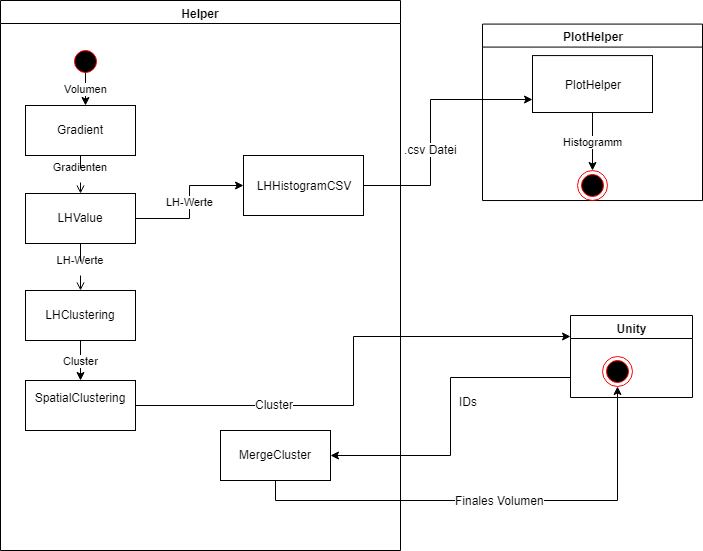
\includegraphics[width=\textwidth]{Logos/Ueberblick.png}
\caption{Überblick über das Programm} 
\label{fig:ueberblick} 
\end{figure}


Damit das Verfahren funktioniert, muss das geladene Volumen als "unsigned int" vorliegen. Der Ablauf der Berechnung startet in der statischen \textit{Gradient} Klasse. Diese ist eine Implementierung des Verfahren von Hong \cite{hong2003method}. Sie nimmt für ihre Berechnung als Parameter ein Volumen von Integern entgegen und gibt ein Volumen mit dem generischen Datentyp \textit{FVector3} zurück. Diese ist eine Hilfsklasse zur Darstellung von dreidimensionalen Vektoren.

Als nächstes wird die Funktion \textit{LHValueVolume} der statischen Klasse \textit{LHValues} aufgerufen. Diese berechnet für das gegebene \textit{FVector3} Volumen und den dazugehörigen Intensitätswerten die LH-Werte für jeden Voxel. Diese gibt die Methode in Form eines Volumens vom Typen "Tuple<float,float>" zurück.

Hat der Benutzer das Modul LHHistogram aufgerufen, entsteht im Anschluss das LH-Histogramm in der Klasse \textit{LHHistogramCSV} und wird von ihr als .csv Datei in einem vom Anwender angegebenen Pfad abgespeichert. Diese kann der Benutzer anschließend in dem Pythonscript \textit{PlotHelper}  laden und sich Visualisieren lassen. Hierbei ist zu beachten, dass das Histogramm gebildet wird, indem die Häufigkeit des Vorkommens eines LH-Wertpaares im Volumen im jeweils dazu passenden Kästchen gespeichert wird. Dies ist simpler als das im Paper von Nguyen \cite{nguyen2012clustering} benutzte Erstellen des Histogramms abhängig von einer für jeden Voxel berechneten Gewichtung. Da die Arbeit an der Implementierung zeitlich beschränkt war, wurde diese Gewichtung, die einzig und allein einer genaueren Darstellung des für das Verfahren irrelevante LH-Histogramm dient, vernachlässigt. Die Gewichtung ist für das Clustering belanglos, da dort ein Histogramm wie oben beschrieben, abhängig von der Häufigkeit der LH-Werte verwendet wird. 


Wurde jedoch das ClusterVolume Modul aufgerufen, wird mit den beiden Clusteringschritten fortgefahren.
Die Berechnung die in der \textit{LHClustering} Klasse geschieht nimmt das Volumen mit den LH-Werten entgegen und rechnet es aus Performancegründen in ein ein Histogramm um. Dieser Schritt könnte gespart werden, wenn die Methode \textit{LHValueVolume} direkt ein Histogramm als Rückgabewert liefern würde. Als Ergebnis der Clusteringfunktion \textit{ComputeLHClusters} wird eine Liste der Cluster zurückgegeben. Ein Cluster besteht aus einer Liste von \textit{IVector3}.Diese Hilfsklasse beschreibt wie \textit{FVector3} Vektoren, jedoch können die Werte nur ganze Zahlen annehmen, folglich eigenen sie sich gut, wie hier verwendet, zum Beschreiben von Positionen im Volumen.Die Cluster werden nur als Liste der räumliche Information der Punkte gespeichert, da für den nächsten Clusteringschritt  lediglich diese Information benötigt wird. 